\documentclass[12pt,a4paper]{report}

% ─── Encodage & langue ───────────────────────────────────────────────────────
\usepackage[utf8]{inputenc}
\usepackage[T1]{fontenc}
\usepackage[provide=*,french]{babel}
\usepackage{csquotes}

% ─── Mise en page ────────────────────────────────────────────────────────────
\usepackage[top=2.5cm, bottom=2.5cm, left=3cm, right=2.5cm]{geometry}
\usepackage{setspace}
\usepackage{wrapfig}
\onehalfspacing

% ─── Typographie ─────────────────────────────────────────────────────────────
\usepackage{lmodern}
\usepackage{microtype}

% ─── Couleurs & graphiques ───────────────────────────────────────────────────
\usepackage[dvipsnames]{xcolor}
\usepackage{graphicx}
\usepackage{float}
\usepackage{caption}
\usepackage{subcaption}

% ─── Tableaux ────────────────────────────────────────────────────────────────
\usepackage{booktabs}
\usepackage{tabularx}
\usepackage{multirow}
\usepackage{array}

% ─── Code source ─────────────────────────────────────────────────────────────
\usepackage{listings}
\usepackage{enumitem}

\lstset{
  basicstyle=\ttfamily\small,
  keywordstyle=\color{blue}\bfseries,
  commentstyle=\color{gray}\itshape,
  stringstyle=\color{red},
  breaklines=true,
  frame=single,
  numbers=left,
  numberstyle=\tiny\color{gray},
  captionpos=b
}

% ─── Mathématiques ───────────────────────────────────────────────────────────
\usepackage{amsmath, amssymb, amsfonts}

% ─── Algorithmes ─────────────────────────────────────────────────────────────
\usepackage{algorithm}
\usepackage{algpseudocode}

% ─── UML / TikZ ──────────────────────────────────────────────────────────────
\usepackage{tikz}
\usetikzlibrary{shapes.geometric, arrows.meta, positioning, fit, backgrounds}

% ─── Diagramme de Gantt ──────────────────────────────────────────────────────
\usepackage{pgfgantt}

% ─── Hyperliens ──────────────────────────────────────────────────────────────
\usepackage[hidelinks, colorlinks=true, linkcolor=NavyBlue, urlcolor=NavyBlue, citecolor=NavyBlue]{hyperref}

% ─── Bibliographie ───────────────────────────────────────────────────────────
\usepackage[backend=biber, style=ieee]{biblatex}
\addbibresource{references.bib}   % décommenter quand le fichier .bib est prêt

% ─── En-têtes / pieds de page ────────────────────────────────────────────────
\usepackage{fancyhdr}
\setlength{\headheight}{14.2pt}
\addtolength{\topmargin}{-2.2pt}
\pagestyle{fancy}
\fancyhf{}
\fancyhead[L]{\small PFE n°1 — MC-SLAM}
\fancyhead[R]{\small \leftmark}
\fancyfoot[C]{\thepage}
\renewcommand{\headrulewidth}{0.4pt}

% ─── Glossaire / acronymes ───────────────────────────────────────────────────
\usepackage[acronym, toc]{glossaries}
\makeglossaries

\newacronym{slam}{SLAM}{Simultaneous Localization and Mapping}
\newacronym{ros}{ROS}{Robot Operating System}
\newacronym{lidar}{LiDAR}{Light Detection And Ranging}
\newacronym{rgb}{RGB}{Red Green Blue}
\newacronym{lwir}{LWIR}{Long Wave InfraRed}
\newacronym{imu}{IMU}{Inertial Measurement Unit}
\newacronym{gs}{3DGS}{3D Gaussian Splatting}
\newacronym{uml}{UML}{Unified Modeling Language}
\newacronym{pfe}{PFE}{Projet de Fin d'Études}

% ─── Informations du document ────────────────────────────────────────────────
\title{
  \vspace{-1cm}
  
\includegraphics[width=4cm]{img/UB.png}\\[1.5cm]
  \Huge\bfseries Rapport de Projet de Fin d'Études\\[0.5cm]
  \large SLAM Multi-Capteurs\\[0.3cm]
  \normalsize\texttt{MC-SLAM}
}
\author{
  \textbf{Matis DUVAL}\\
}
\date{Année universitaire 2025--2026}

\begin{document}

\maketitle
\thispagestyle{empty}

\begin{abstract}
  Ce rapport présente le travail réalisé dans le cadre du \acrfull{pfe} intitulé
  \emph{SLAM Multi-Capteurs (MC-SLAM)}. L'objectif principal est la prise en main
  de la plateforme TurtleBot~4 sous \acrfull{ros}~2, suivi du développement d'une
  solution de \acrfull{slam} exploitant un \acrshort{lidar} avec l'aide d'autres
  capteurs pour améliorer la précision.
\end{abstract}

\newpage

\tableofcontents
\listoffigures
\listoftables
\printglossary[type=\acronymtype, title=Liste des acronymes]

\newpage

\chapter{Introduction}

\section{Contexte}

La robotique mobile autonome connaît un essor considérable, portée par les
avancées en intelligence artificielle, en vision par ordinateur et en capteurs
embarqués. Dans ce contexte, la capacité d'un robot à se localiser tout en
construisant une carte de son environnement --- le \acrfull{slam} --- est
devenu une brique fondamentale de nombreuses applications~: navigation en
intérieur, véhicules autonomes, inspection industrielle ou encore robotique de
service.

Ce projet vise à exploiter la plateforme robotique \textbf{TurtleBot~4} pour
développer et comparer différentes approches de \acrshort{slam} multi-capteurs.

\section{Problématique}

Malgré l'avancée des algorithmes de \acrshort{slam} monoculaires ou
monocapteurs, plusieurs problèmes subsistent~:

\begin{itemize}
  \item \textbf{Mauvaises conditions d'éclairage}~: les approches
        \acrshort{rgb} sont sensibles aux variations lumineuses~; les capteurs
        \acrshort{lwir} offrent une alternative thermique mais restent peu
        explorés dans ce contexte.
  \item \textbf{Fusion multi-capteurs}~: la combinaison \acrshort{lidar} +
        caméra peut améliorer la précision, mais nécessite une calibration.
  \item \textbf{Vitesse de traitement}~: la plateforme TurtleBot~4 est
        limitée en ressources, ce qui impose des algorithmes efficaces pour le
        temps réel.
\end{itemize}

\section{Sujet et objectifs}

Les objectifs du projet sont les suivants~:

\begin{enumerate}
  \item \textbf{Prise en main} de la plateforme TurtleBot~4 (architecture
        matérielle, logicielle sous \acrshort{ros}~2, calibration des capteurs).
  \item \textbf{Développement d'un pipeline MC-SLAM} exploitant la caméra
        \acrshort{rgb} et le \acrshort{lidar} intégré.
  \item \textbf{Comparaison des performances} du SLAM LiDAR
        et évaluation de l'apport de la fusion multi-capteurs.
\end{enumerate}

\chapter{État de l'art}

\section{SLAM visuel (Visual SLAM)}

Le SLAM visuel utilise des caméras comme capteur principal. Parmi les systèmes
les plus répandus, ORB-SLAM3 propose une architecture complète supportant les
caméras monoculaire, stéréo et RGB-D, avec une gestion de la réinitialisation
et des cartes multi-sessions~\cite{campos2021orbslam3}. DSO (\emph{Direct
  Sparse Odometry}) adopte quant à lui une approche directe fondée sur la
minimisation de l'erreur photométrique, ce qui le rend particulièrement adapté
aux scènes peu texturées ou aux environnements où les données d'autres capteurs
sont peu fiables. Enfin, VINS-Mono et VINS-Fusion intègrent la vision et une
centrale inertielle (\acrshort{imu}) afin de fournir une odométrie
visuo-inertielle précise.

\section{SLAM LiDAR}

Les approches LiDAR offrent une précision métrique supérieure en extérieur et
dans les larges espaces. LOAM et sa variante légère LeGO-LOAM reposent sur
l'extraction de \emph{features} géométriques des arêtes et plans pour assurer
l'odométrie et la cartographie en temps réel. LIO-SAM étend cette approche en
fusionnant les données LiDAR et \acrshort{imu} au sein d'une optimisation par
graphe de facteurs. À l'opposé, KISS-ICP propose un pipeline minimaliste et
robuste basé sur l'ICP adaptatif, particulièrement adapté aux plateformes
embarquées~\cite{vizzo2023kissICP}.

\section{SLAM multi-capteurs}

La fusion de plusieurs modalités permet de combiner leurs forces respectives.
Les travaux récents s'appuient sur des graphes de facteurs (GTSAM, g2o) pour
intégrer des contraintes hétérogènes (LiDAR, caméra, \acrshort{imu}, GPS).

\section{SLAM thermique (LWIR)}

Le SLAM basé sur caméra \acrshort{lwir} est un domaine émergent. Les images
thermiques sont invariantes aux conditions d'éclairage visible, ce qui les rend
attractives pour les environnements obscurs ou enfumés. Cependant, leur faible
résolution et le manque de texture fine posent des défis pour l'extraction de
\emph{keypoints}. Des avancées récentes comme le Thermal-SLAM réduisent
l'impact du bruit thermique et améliorent la détection de
\emph{features}~\cite{wu2023thermalslam}.

\section{3D Gaussian Splatting}

Introduit par Kerbl \emph{et al.}~(2023), le \acrfull{gs} représente une scène
3D par un ensemble de gaussiennes 3D anisotropes, permettant un rendu en temps
réel de haute qualité. Son intégration dans un pipeline SLAM (\emph{SplaTAM},
\emph{MonoGS}) ouvre la voie à des cartes denses et
photo-réalistes~\cite{kerbl2023gaussian}.

\chapter{User Stories}

Les \emph{user stories} suivantes ont été définies par mes soins pour permettre
une meilleure compréhension de l'objectif principal et afin de créer un Kanban.

\begin{table}[H]
  \centering
  \caption{User stories principales}\label{tab:user_stories}
  \renewcommand{\arraystretch}{1.4}
  \begin{tabularx}{\textwidth}{c l X c}
    \toprule
    \textbf{ID} & \textbf{Rôle} & \textbf{Objectif}                                                 & \textbf{Priorité} \\
    \midrule
    US-01       & Développeur   & Comprendre l'architecture matérielle et logicielle du TurtleBot~4
                & Haute                                                                                                 \\
    US-02       & Développeur   & Calibrer la caméra RGB et le LiDAR (intrinsèque +
    extrinsèque)
                & Haute                                                                                                 \\
    US-03       & Développeur   & Lancer un pipeline SLAM RGB et visualiser la carte en
    temps réel dans RViz2
                & Haute                                                                                                 \\
    US-04       & Développeur   & Lancer un pipeline SLAM LiDAR et comparer la précision
    avec US-03
                & Haute                                                                                                 \\
    US-05       & Développeur   & Fusionner les données RGB + LiDAR pour améliorer la
    robustesse du SLAM
                & Moyenne                                                                                               \\
    \bottomrule
  \end{tabularx}
\end{table}

\chapter{Spécification des besoins}

\section{Besoins fonctionnels}

\begin{enumerate}[label=\textbf{BF-\arabic*}]
  \item Le système doit permettre le pilotage du TurtleBot-4 via une téléopération
        \acrshort{ros}~2 clavier.
  \item Le système doit acquérir et synchroniser les flux de données de la caméra RGB-D
        (OAK-D Pro) et du LiDAR (RPLiDAR A1M8).
  \item Le système doit réaliser la calibration intrinsèque et extrinsèque de la caméra
        et du LiDAR.\@
  \item Le système doit exécuter un algorithme de SLAM RGB en temps réel et publier la
        carte et la pose estimée sur les topics ROS~2 adéquats.
  \item Le système doit exécuter un algorithme de SLAM LiDAR en temps réel.
\end{enumerate}

\section{Tests}
Les tests n'ont pas été effectués avec l'outil
\texttt{rpg\_trajectory\_evaluation} mais une évaluation qualitative a été
faite en comparant les cartes obtenues par le pipeline SLAM LiDAR.\@ En effet,
le temps limité du projet ne m'a pas permis de réaliser une évaluation
quantitative avec les outils demandés. Cependant, les cartes produites
attestent que le robot arrive au moins à reconstruire une carte cohérente de
son environnement.
\begin{description}
  \item[rpg\_trajectory\_evaluation] Outil pour l'évaluation de la précision de
        l'odométrie LiDAR, disponible à l'adresse
        \url{https://github.com/uzh-rpg/rpg_trajectory_evaluation}.
\end{description}

\chapter{Choix logiciels}
Ce chapitre présente l'ensemble des outils, bibliothèques et langages retenus
pour le développement. Les choix ont été faits en fonction de leur
compatibilité avec ROS~2 Jazzy et de leur facilité d'intégration dans le
projet.

\section{Système d'exploitation et middleware}
Le système d'exploitation s'impose de lui-même~: pour assurer la bonne
continuité du projet et éviter les problèmes de compatibilité, il faut choisir
un système d'exploitation compatible avec ROS~2 Jazzy.

\begin{description}
  \item[Ubuntu 22.04 LTS] Distribution de référence pour ROS~2 Jazzy, bénéficiant d'un
        support long terme.
  \item[ROS~2 Jazzy] Version LTS de ROS~2 offrant une architecture DDS fiable, des
        outils de débogage matures (RViz2, rqt, ros2bag) et une compatibilité native
        avec TurtleBot~4.
\end{description}

\section{Algorithmes de SLAM}
Le SLAM a été implémenté ''from scratch'' pour le LiDAR (ICP) et la calibration
extrinsèque, afin de mieux comprendre les algorithmes de base.

\begin{description}
  \item[ICP] Implémenté à partir de zéro pour l'odométrie LiDAR, en utilisant une
        approche de correspondance de points et d'estimation de transformation rigide.
  \item[Bresenham] Utilisé pour trouver les correspondances entre les points du LiDAR
        et les pixels.
  \item[ORB] Utilisé pour l'extraction de \emph{keypoints} et de descripteurs dans les
        images RGB pour la fermeture de boucle visuelle.
\end{description}

\section{Calibration}
La calibration de la caméra n'a pas été l'objectif principal du projet~; le
choix d'utiliser une solution existante a donc été fait pour gagner du temps et
se concentrer sur le SLAM.\@

\begin{description}
  \item[camera\_calibration (ROS~2)] Calibration intrinsèque caméra via damier imprimé,
        avec support pour les caméras RGB.\@
\end{description}

L'outil de calibration ROS n'étant plus à jour pour les nouveaux modèles de
TurtleBot, il a fallu développer un nœud ROS pour pousser les données de
calibration vers la caméra.\@

\section{Développement et versioning}

\begin{description}
  \item[Git + GitHub] Versioning et collaboration.
  \item[Gazebo] Simulateur de robotique 3D pour les tests préliminaires en simulation
        avant déploiement sur le robot réel. Le TurtleBot~4 dispose d'ailleurs d'une
        simulation officielle.
  \item[Colcon] Outil de build recommandé pour ROS~2, facilitant la gestion des
        dépendances et l'organisation du workspace.
  \item[Python 3.10 et OpenCV] Langage de programmation utilisé pour le pipeline caméra
        avec OpenCV.\@
  \item[C++] Langage de programmation pour le LiDAR ICP, offrant de meilleures
        performances.
  \item[LLMs (Claude, Gemini)] Utilisés pour la génération de code, la rédaction de
        documentation et l'assistance à la résolution de problèmes.
\end{description}

\chapter{Architecture}

\section{Architecture matérielle}

La plateforme TurtleBot~4 est composée des éléments matériels suivants~:

\begin{itemize}
  \item \textbf{Base iRobot Create~3}~: plateforme de déplacement différentiel
        avec encodeurs et \acrshort{imu} intégrés.
  \item \textbf{Raspberry Pi~4B (4~Go)}~: calculateur embarqué principal.
  \item \textbf{Caméra OAK-D Pro}~: caméra RGB-D stéréo avec accélérateur
        neural intégré (Intel MyriadX).
  \item \textbf{LiDAR RPLiDAR A1M8}~: scanner laser 2D 360° à 12~Hz.
  \item \textbf{IMU}~: intégrée à la base iRobot, fournissant des mesures d'accélération et de
        rotation.
\end{itemize}

\section{Architecture logicielle ROS 2}

L'architecture logicielle du projet est organisée en plusieurs nœuds ROS~2
communicants via des topics et des services~:

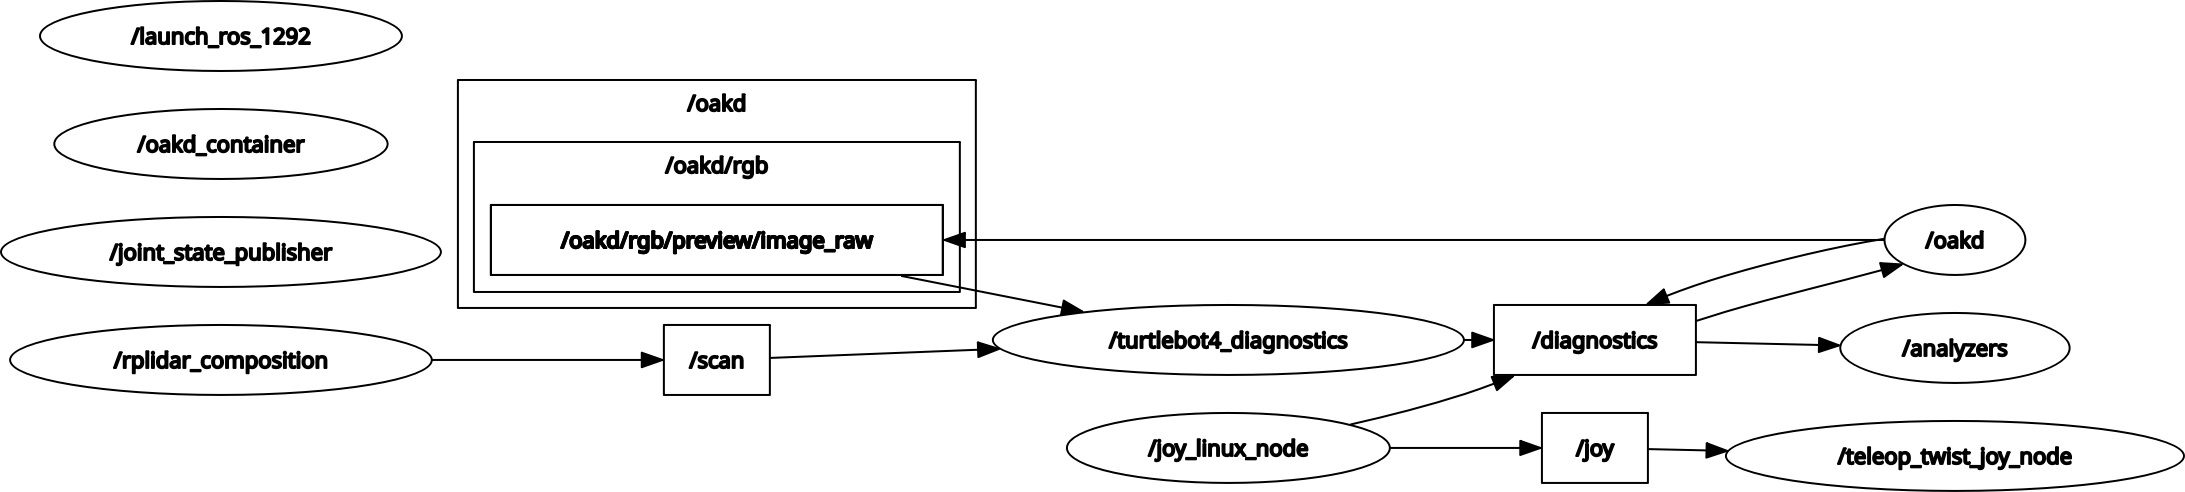
\includegraphics[width=\textwidth]{img/rosgraph.png}

\section{Diagramme de cas d'utilisation (UML)}

%Redo UML
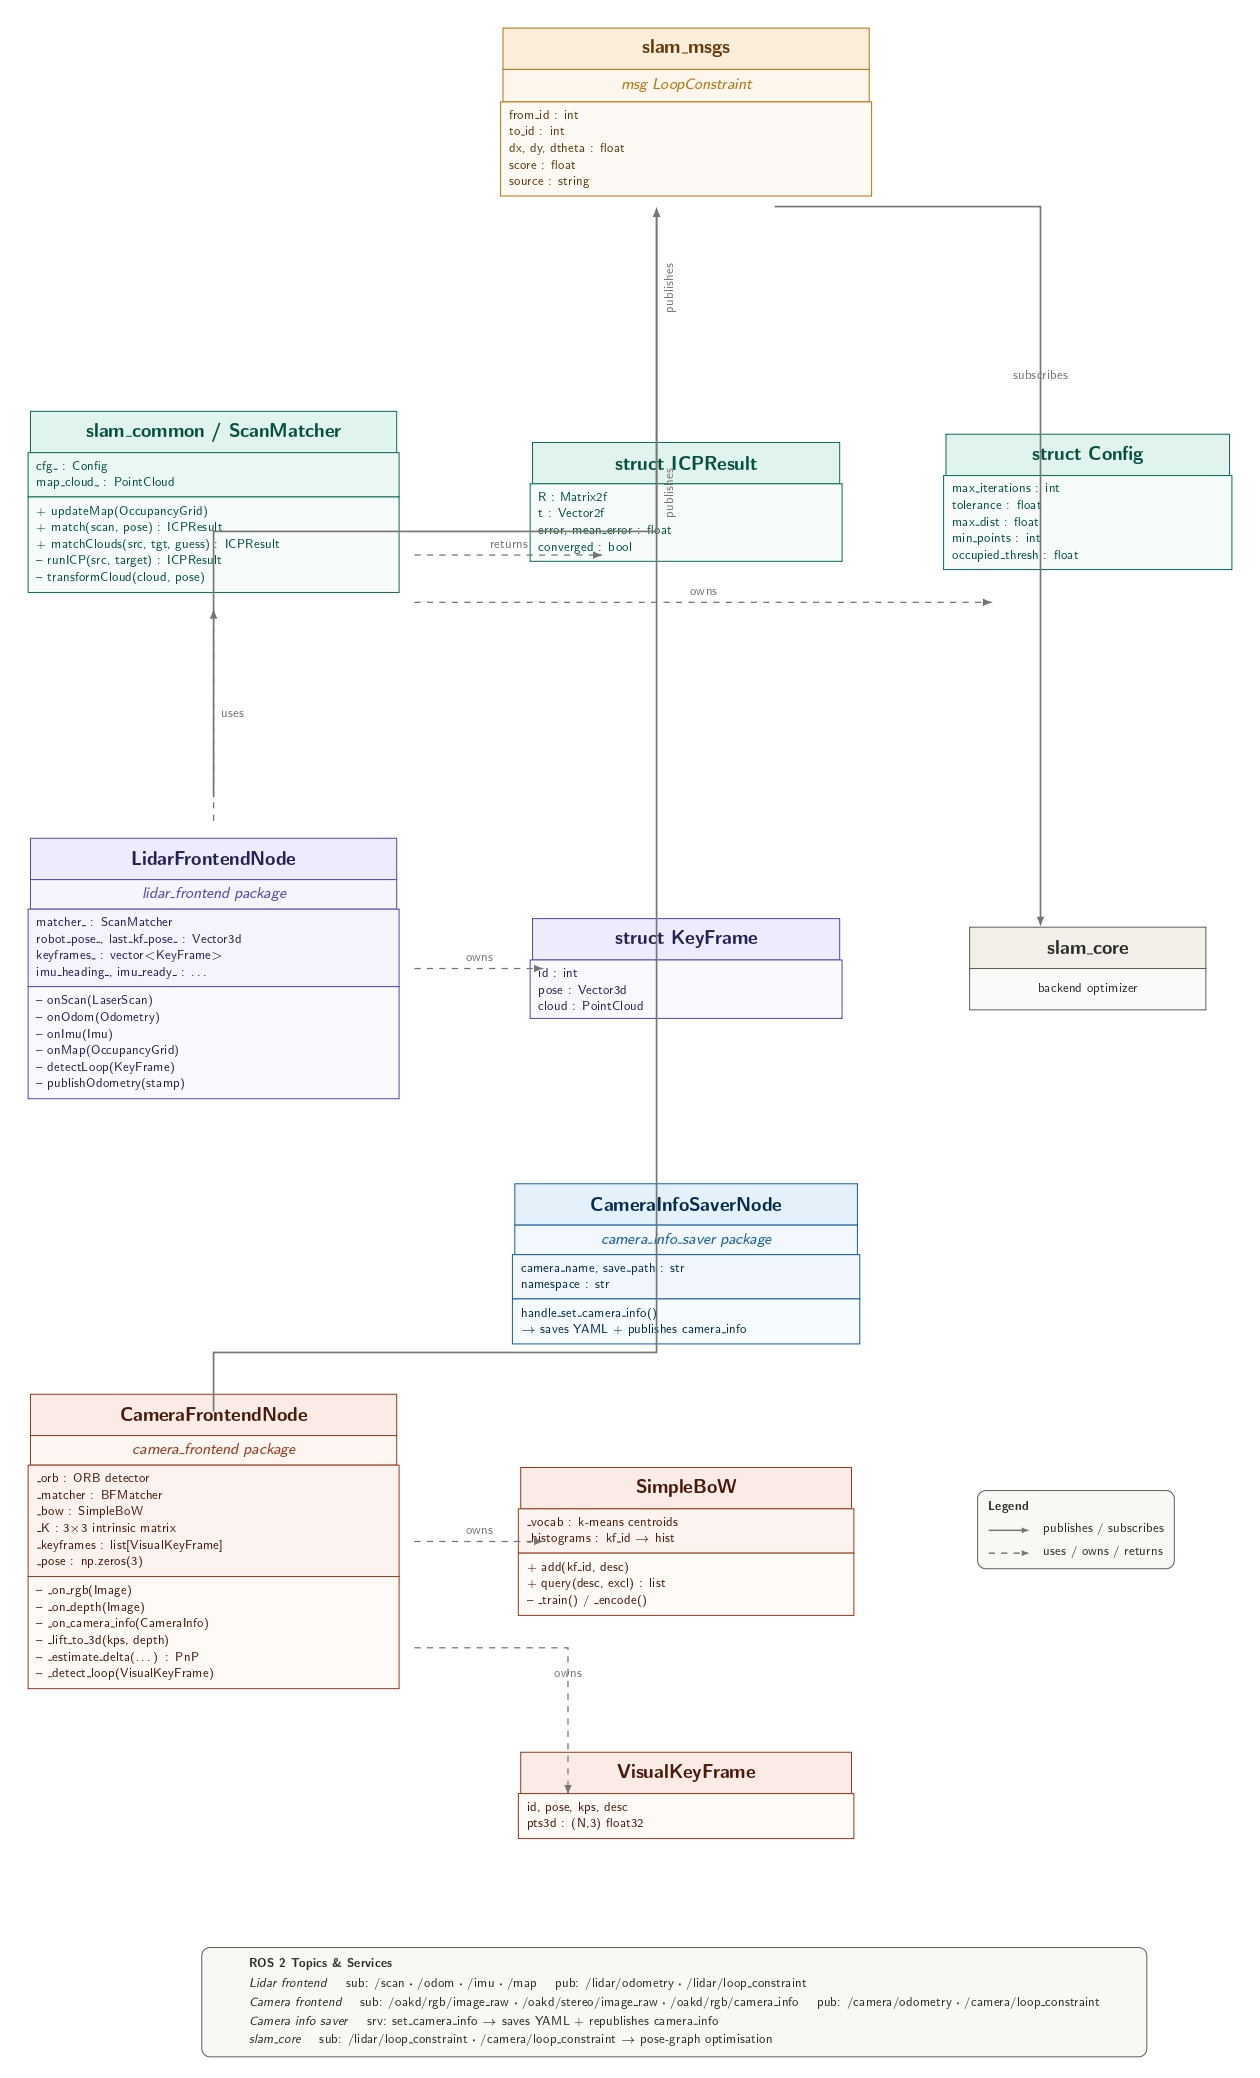
\includegraphics[width=\textwidth]{img/slam_uml.jpg}

\chapter{Réalisation}

\section{Mise en place de l'environnement}

L'environnement de développement a été configuré comme suit~:

\begin{lstlisting}[language=bash, caption={Installation de l'environnement ROS 2 et TurtleBot 4}]
sudo apt update && sudo apt install ros-jazzy-desktop -y

sudo apt install ros-jazzy-turtlebot4-desktop -y

git clone https://github.com/xdZireael/PFE

cd PFE_ws && colcon build --symlink-install

source install/setup.bash
\end{lstlisting}

\section{Captures d'écran}\label{sec:screenshots}

\begin{figure}[H]
  \centering
  \begin{subfigure}{0.48\textwidth}
    \centering
    %Better screens
    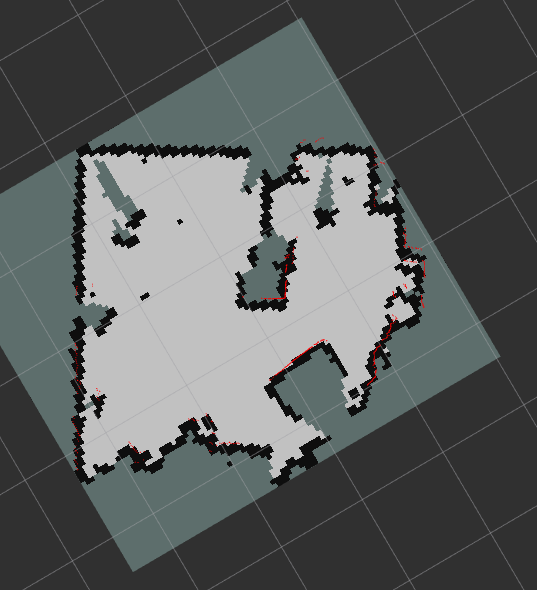
\includegraphics[width=\textwidth]{img/benchmap.png}
    \caption{Carte SLAM benchmark dans RViz2}\label{fig:rviz_rgb}
  \end{subfigure}
  \hfill
  \begin{subfigure}{0.48\textwidth}
    \centering
    %Better screens
    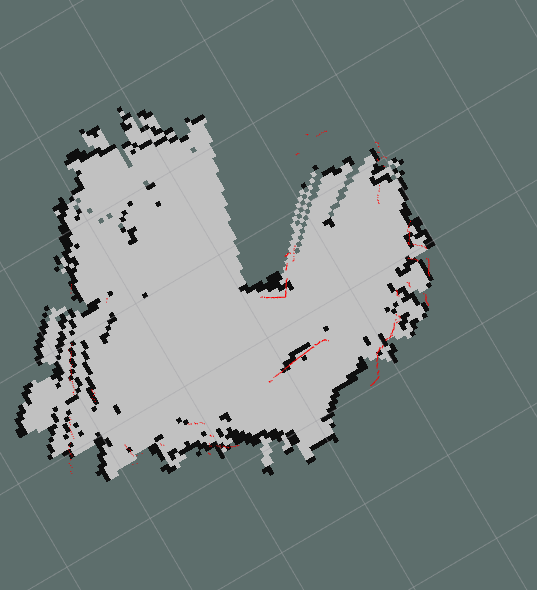
\includegraphics[width=\textwidth]{img/lidarmap.png}
    \caption{Carte SLAM LiDAR dans RViz2}\label{fig:rviz_lidar}
  \end{subfigure}
  \caption{Visualisation des cartes générées par les deux pipelines SLAM}\label{fig:rviz_comparaison}
\end{figure}

\section{Algorithmes et méthodes}
\subsection{ICP implémenté de zéro}

L'algorithme ICP est décrit ci-dessous~:

\begin{algorithm}[H]
  \caption{ICP (Iterative Closest Point) pour l'odométrie LiDAR}\label{alg:icp}
  \begin{algorithmic}[1]
    \Require $P = \{p_i\}$, $Q = \{q_j\}$ (nuages de points source et cible)
    \Ensure Transformation rigide $T \in SE(3)$ alignant $P$ sur $Q$
    \State Initialiser $T \gets I$ (identité)
    \Repeat
    \State Trouver les correspondances $C = \{(p_i, q_j)\}$
    \State Estimer la transformation $T$ minimisant l'erreur de correspondance~:
    \[
      T = \arg\min_{T} \sum_{(p_i, q_j) \in C} \| T p_i - q_j \|^2
    \]
    \State Appliquer $T$ à $P$~: $P \gets T P$
    \Until{convergence (changement de $T$ inférieur à un seuil) ou nombre maximal d'itérations atteint}
  \end{algorithmic}
\end{algorithm}

\begin{algorithm}[H]
  \caption{Détection de fermeture de boucle LiDAR avec une pipeline à trois verrous}\label{alg:lidar-lc}
  \begin{algorithmic}[1]
    \Require Image courante de keyframe $\mathbf{k}_{\text{cur}}$ avec sa pose $\mathbf{p}_{\text{cur}}$
    et son nuage de points $\mathcal{P}_{\text{cur}}$,
    historique de keyframes $\{\mathbf{k}_i\}_{i=0}^{n-1}$,
    rayon de recherche spatiale $r_{\text{lc}} = 1.0\,\text{m}$,
    âge minimal de séparation $A = 5$ keyframes pour éviter les faux positifs immédiats,
    seuil de qualité ICP $\tau_{\text{icp}} = 0.10\,\text{m}$,
    distance maximale d'inlier $d_{\text{in}} = 0.10\,\text{m}$,
    ratio minimal d'inliers $\rho_{\min} = 0.65$
    \Ensure  Message de contrainte de boucle, ou absence de boucle détectée

    \For{chaque keyframe candidate $\mathbf{k}_i$ avec $i < n_{\text{cur}} - A$}

    \State \textbf{Verrou 1 — proximité spatiale.}
    Calculer la distance euclidienne entre la position courante et la position de la candidate.
    Rejeter immédiatement si la distance dépasse le rayon de recherche $r_{\text{lc}}$,
    ce qui évite tout recalage ICP coûteux sur des paires éloignées.

    \State \textbf{Verrou 2 — recalage ICP entre les deux nuages.}
    Construire une pose relative initiale à partir des poses stockées des deux keyframes,
    puis lancer l'ICP (Algorithme~\ref{alg:icp}) entre $\mathcal{P}_{\text{cur}}$ et $\mathcal{P}_i$.
    Rejeter la candidate si l'ICP n'a pas convergé ou si l'erreur résiduelle dépasse $\tau_{\text{icp}}$~:
    \[
      (\mathbf{R},\, \mathbf{t},\, \bar{e},\, \text{conv})
      \gets \mathrm{ICP}(\mathcal{P}_{\text{cur}},\; \mathcal{P}_i,\; \Delta\mathbf{p})
    \]

    \State \textbf{Verrou 3 — test du ratio d'inliers.}
    Appliquer la transformation ICP à chaque point du nuage courant,
    puis compter les points dont le voisin le plus proche dans $\mathcal{P}_i$
    est à moins de $d_{\text{in}}$. Ce test détecte les convergences ICP spurieuses
    vers un minimum local géométriquement plausible mais physiquement incorrect~:
    \[
      \rho \gets \frac{\#\left\{\mathbf{s} \in \mathcal{P}_{\text{cur}} \;\middle|\;
      \min_{j}\|\mathbf{R}\mathbf{s} + \mathbf{t} - \mathbf{t}_j\| < d_{\text{in}}\right\}}
      {|\mathcal{P}_{\text{cur}}|}
    \]
    Rejeter si $\rho < \rho_{\min}$.

    \State \textbf{Les trois verrous sont passés.}
    Émettre le message de contrainte de boucle avec l'identifiant de la keyframe source,
    l'identifiant de la keyframe cible, le déplacement relatif $(\mathbf{t},\, \Delta\theta)$
    déduit de $\mathbf{R}$, et le score de qualité $\bar{e}$.
    Retourner immédiatement (une seule boucle par keyframe).

    \EndFor

    \State Aucune fermeture de boucle détectée pour cette keyframe
  \end{algorithmic}
\end{algorithm}

\begin{algorithm}[H]
  \caption{EKF — étape de correction par mesure de pose (LiDAR ou caméra)}\label{alg:ekf-update}
  \begin{algorithmic}[1]
    \Require Moyenne prédite $\boldsymbol{\mu}^-$ et covariance prédite $\boldsymbol{\Sigma}^-$,
    mesure de pose $\mathbf{z} = (x_z, y_z, \theta_z)^\top$ issue du frontend LiDAR ou caméra,
    matrice de bruit de mesure $\mathbf{R}$ propre au capteur
    (LiDAR~: $\sigma_{xy} = 0.03\,\text{m}$, $\sigma_\theta = 0.02\,\text{rad}$~;
    caméra~: $\sigma_{xy} = 0.05\,\text{m}$, $\sigma_\theta = 0.03\,\text{rad}$)
    \Ensure  Moyenne corrigée $\boldsymbol{\mu}$ et covariance corrigée $\boldsymbol{\Sigma}$

    \State Calculer la matrice d'innovation $\mathbf{S}$, somme de la covariance prédite et du bruit de mesure.
    Le modèle d'observation étant l'identité ($\mathbf{H} = \mathbf{I}_3$), il n'y a pas de projection~:
    \[
      \mathbf{S} \gets \boldsymbol{\Sigma}^- + \mathbf{R}
    \]

    \State Calculer le gain de Kalman $\mathbf{K}$, qui pondère la confiance accordée à la mesure
    par rapport à la prédiction~:
    \[
      \mathbf{K} \gets \boldsymbol{\Sigma}^-\, \mathbf{S}^{-1}
    \]

    \State Calculer le vecteur d'innovation $\boldsymbol{\nu}$, écart entre la mesure et la prédiction.
    La composante angulaire est ramenée dans $(-\pi, \pi]$ pour gérer les discontinuités à $\pm\pi$~:
    \[
      \boldsymbol{\nu} \gets \mathbf{z} - \boldsymbol{\mu}^-, \qquad
      \nu_\theta \gets \mathrm{wrapToPi}(\nu_\theta)
    \]

    \State Corriger la moyenne en appliquant le gain au vecteur d'innovation,
    puis normaliser l'angle résultant~:
    \[
      \boldsymbol{\mu} \gets \boldsymbol{\mu}^- + \mathbf{K}\,\boldsymbol{\nu}, \qquad
      \theta \gets \mathrm{wrapToPi}(\theta)
    \]

    \State Réduire la covariance pour refléter le gain d'information apporté par la mesure~:
    \[
      \boldsymbol{\Sigma} \gets (\mathbf{I}_3 - \mathbf{K})\,\boldsymbol{\Sigma}^-
    \]

    \State \Return la moyenne corrigée $\boldsymbol{\mu}$ et la covariance corrigée $\boldsymbol{\Sigma}$
  \end{algorithmic}
\end{algorithm}

\subsection{Calibration extrinsèque caméra/LiDAR}

La calibration extrinsèque consiste à estimer la transformation rigide
${}^L\mathbf{T}_C \in SE(3)$ entre le repère LiDAR $\mathcal{F}_L$ et le repère
caméra $\mathcal{F}_C$~:

\begin{equation}
  {}^L\mathbf{T}_C =
  \begin{bmatrix} \mathbf{R} & \mathbf{t} \\ \mathbf{0}^\top & 1 \end{bmatrix}
  \in SE(3)
\end{equation}

\chapter{Résultats et tests}

\section{Description de l'environnement de test}

Tous les tests ont été réalisés dans mon bureau, une pièce de 10~m$^2$.
Ci-dessous figure un benchmark de la carte générée par les outils TurtleBot~4.

\begin{figure}[H]
  \centering
  \begin{minipage}{0.45\textwidth}
    \centering
    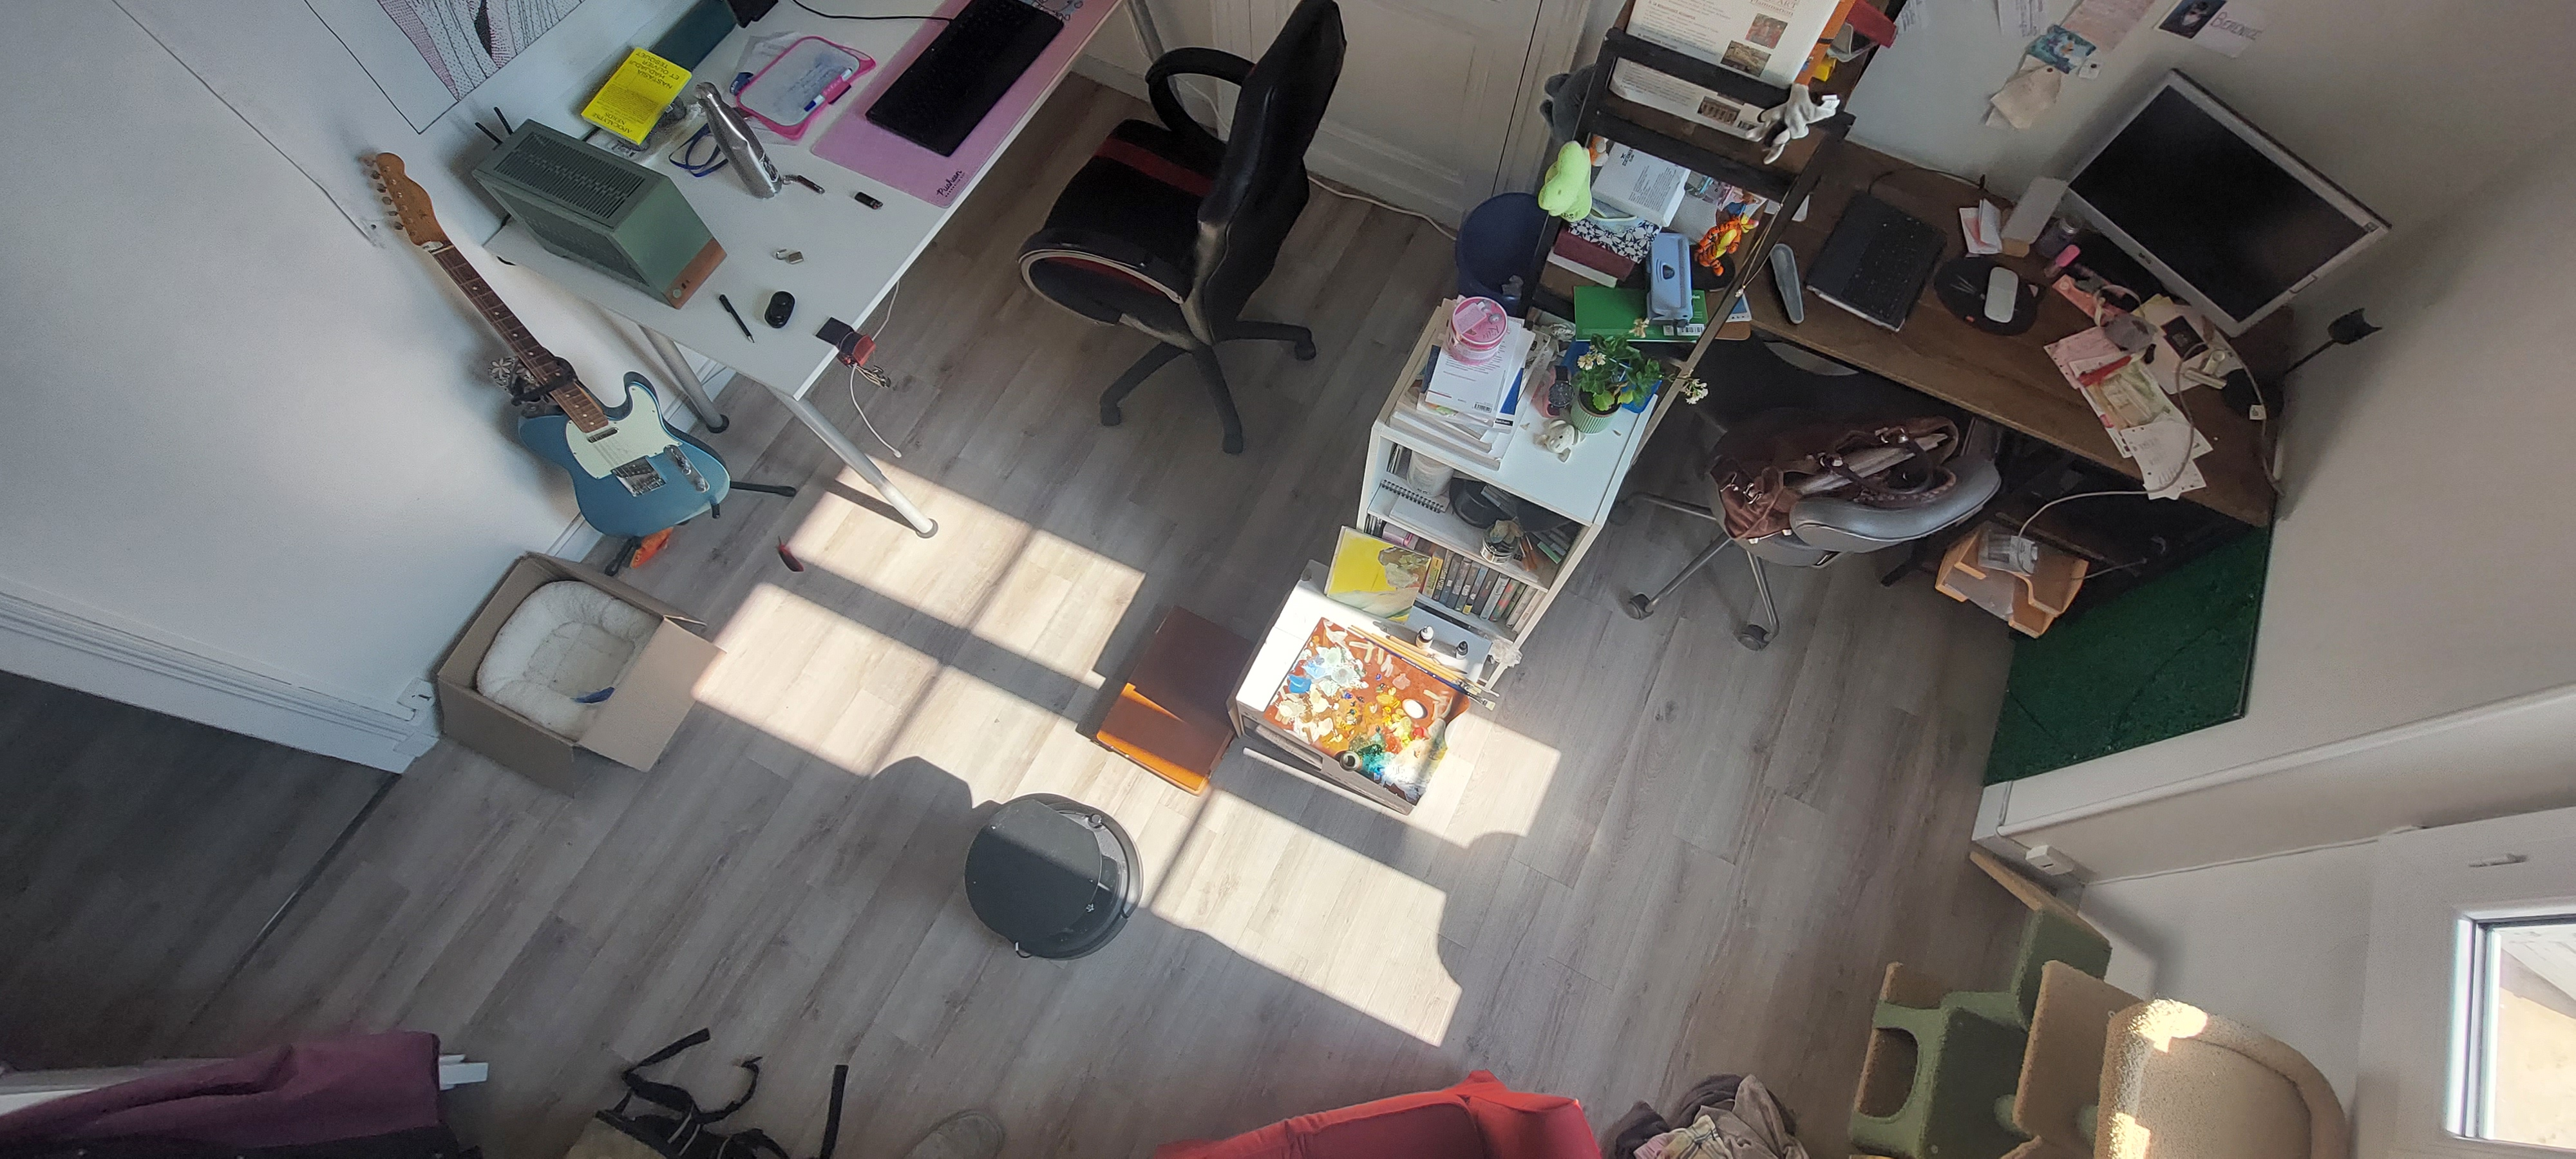
\includegraphics[width=\textwidth]{img/bureau_benchmark_real.jpg}
    \caption{Photo du bureau utilisé pour les tests}
  \end{minipage}
  \hfill
  \begin{minipage}{0.45\textwidth}
    \centering
    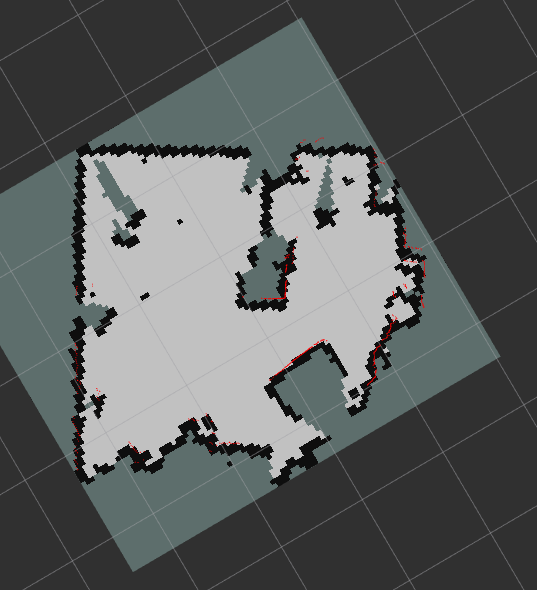
\includegraphics[width=\textwidth]{img/benchmap.png}
    \caption{Carte obtenue par slam-toolbox sur la pièce de bureau}
  \end{minipage}
\end{figure}

\section{Résultats}
Les packages ROS~2 développés permettent une modularité des pipelines SLAM et
donc une visualisation cohérente dans RViz2. Ci-dessous figurent les cartes
obtenues par les pipelines SLAM RGB et LiDAR.\@

Pour chaque cas de test, voici le parcours réalisé par le robot~:
\begin{figure}[H]
  \centering
  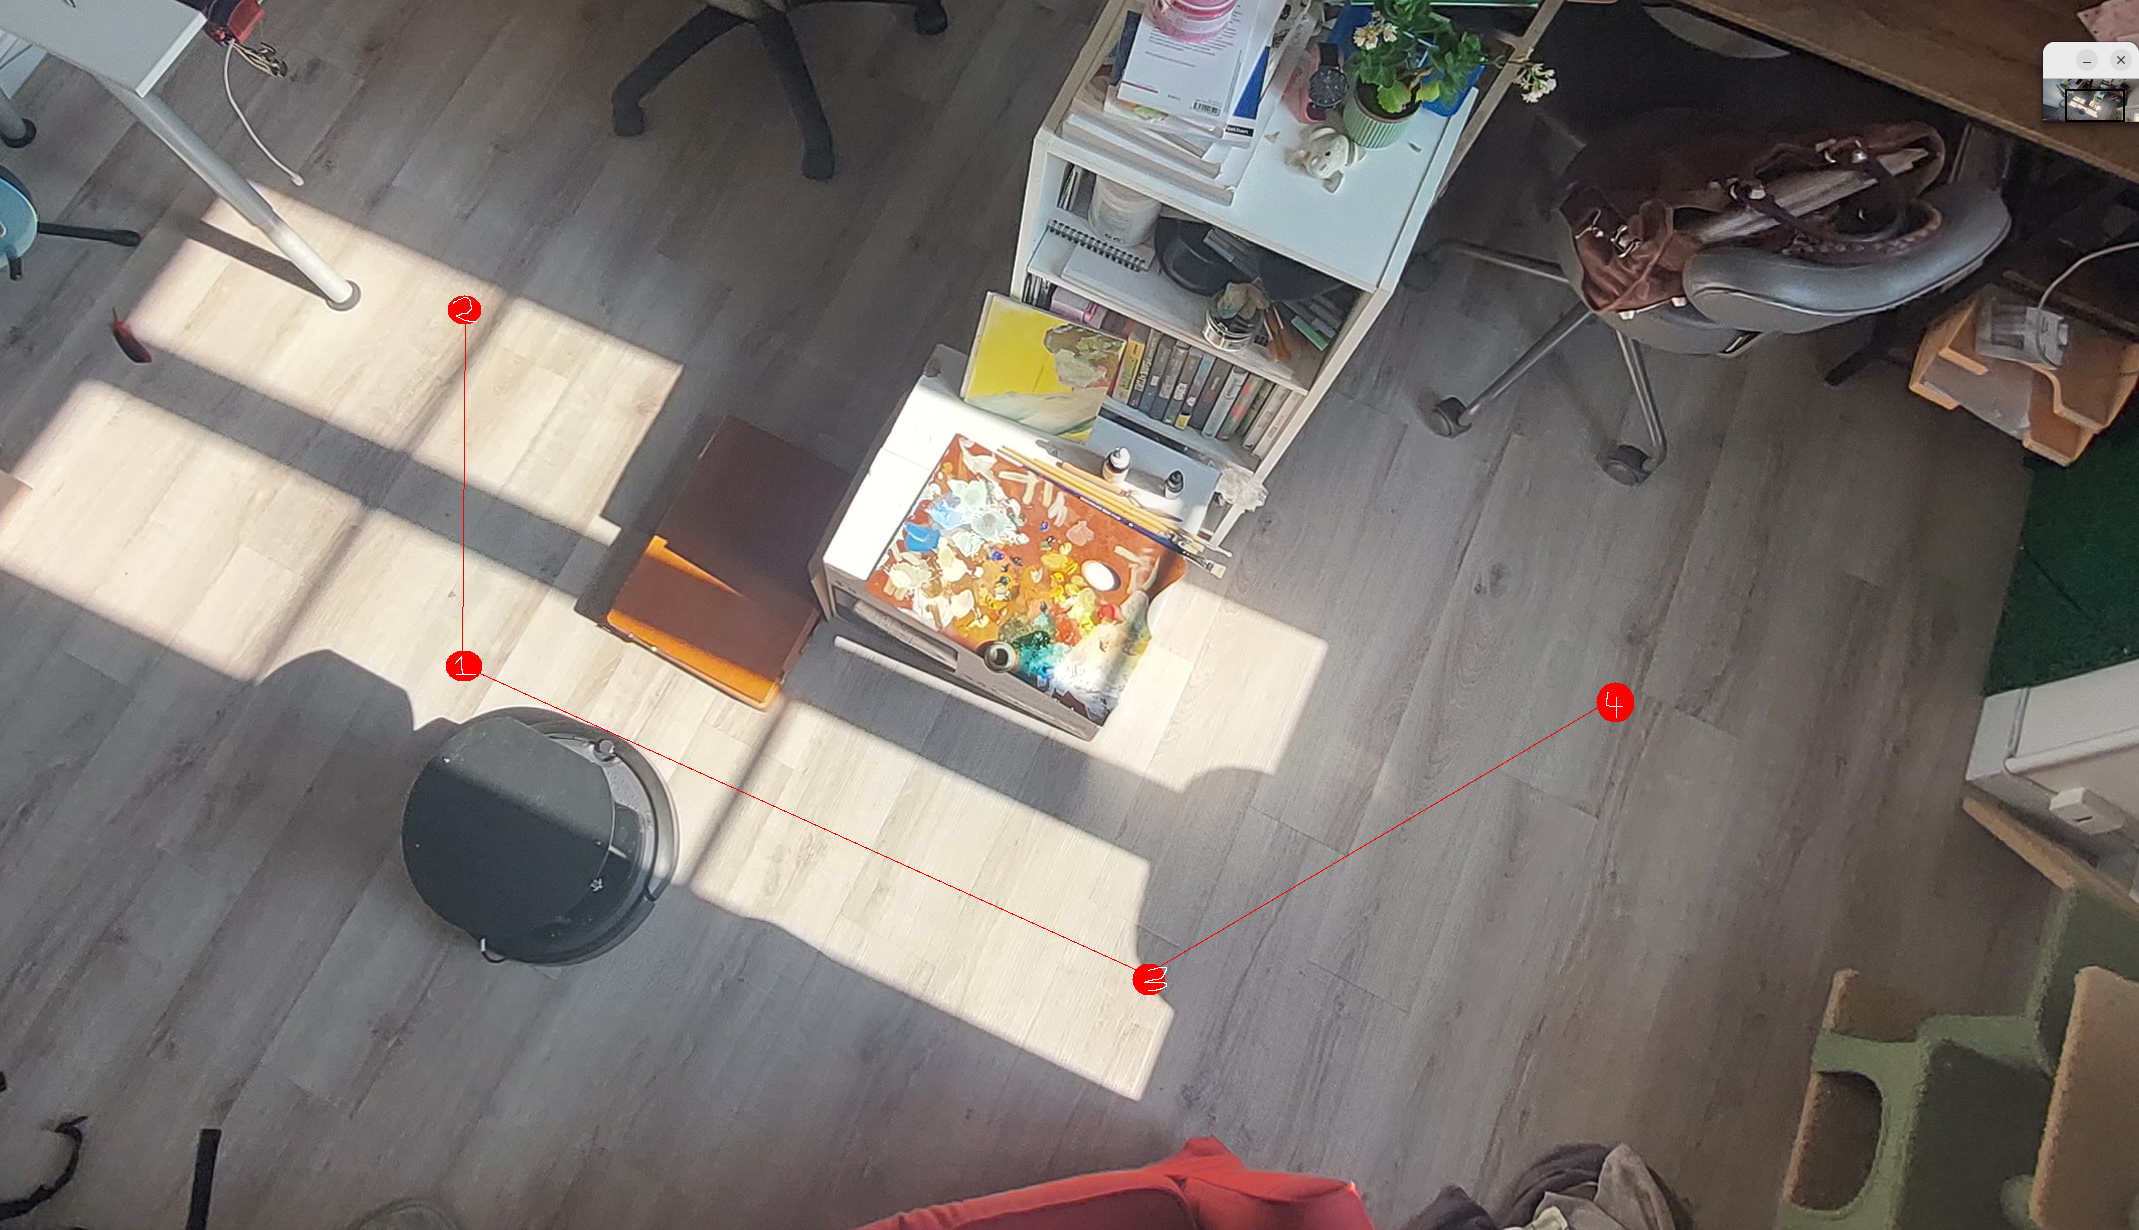
\includegraphics[width=0.8\textwidth]{img/testpath.png}
  \caption{Parcours réalisé par le robot pour les tests SLAM}
\end{figure}

\begin{table}[H]
  \centering
  \caption{Composants actifs du pipeline SLAM}\label{tab:results}
  \renewcommand{\arraystretch}{1.3}
  \begin{tabularx}{\textwidth}{c c c c c}
    \toprule
    \textbf{Test ID} & \textbf{LiDAR} & \textbf{Loop Closure LiDAR} & \textbf{Loop Closure RGB} & \textbf{Fusion} \\
    \midrule
    01               & \checkmark     & \checkmark                  & \checkmark                & \checkmark      \\
    \bottomrule
  \end{tabularx}
\end{table}
\begin{figure}[H]
  \centering
  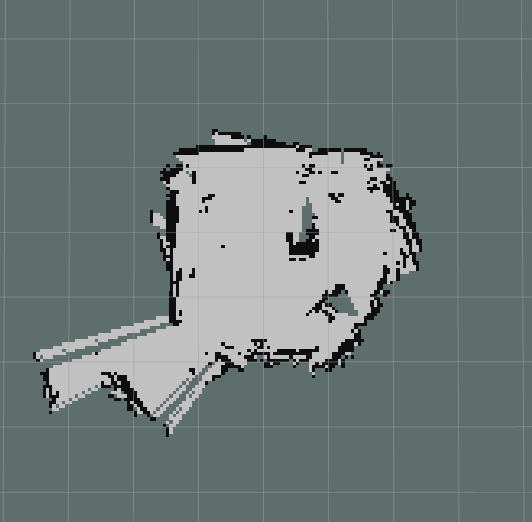
\includegraphics[width=0.6\textwidth]{img/lidarcameraclosuremap.png}
  \caption{Carte MC-SLAM dans RViz2}
\end{figure}

\begin{table}[H]
  \centering
  \caption{Composants actifs du pipeline SLAM (sans RGB)}\label{tab:results-lidar}
  \renewcommand{\arraystretch}{1.3}
  \begin{tabularx}{\textwidth}{c c c c c}
    \toprule
    \textbf{Test ID} & \textbf{LiDAR} & \textbf{Loop Closure LiDAR} & \textbf{Loop Closure RGB} & \textbf{Fusion} \\
    \midrule
    02               & \checkmark     & \checkmark                  &                           &                 \\
    \bottomrule
  \end{tabularx}
\end{table}
\begin{figure}[H]
  \centering
  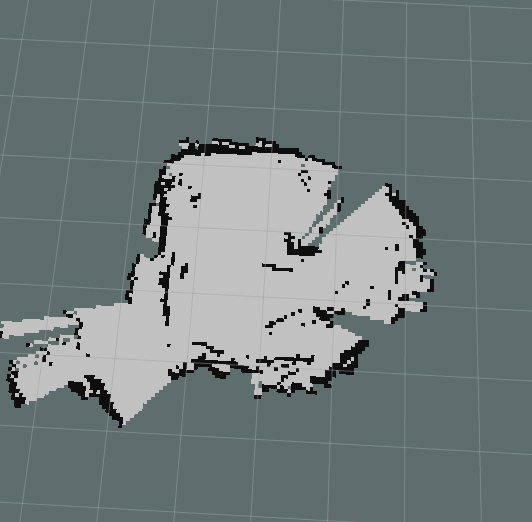
\includegraphics[width=0.6\textwidth]{img/lidarnocammap.png}
  \caption{Carte SLAM sans fermeture de boucle RGB dans RViz2}
\end{figure}

\begin{table}[H]
  \centering
  \caption{Composants actifs du pipeline SLAM (sans fermeture de boucle LiDAR)}\label{tab:results-noicp}
  \renewcommand{\arraystretch}{1.3}
  \begin{tabular}{c c c c c}
    \toprule
    \textbf{Test ID} & \textbf{LiDAR} & \textbf{Loop Closure LiDAR} & \textbf{Loop Closure RGB} & \textbf{Fusion} \\
    \midrule
    04               & \checkmark     &                             & \checkmark                &                 \\
    \bottomrule
  \end{tabular}
\end{table}
\begin{figure}[H]
  \centering
  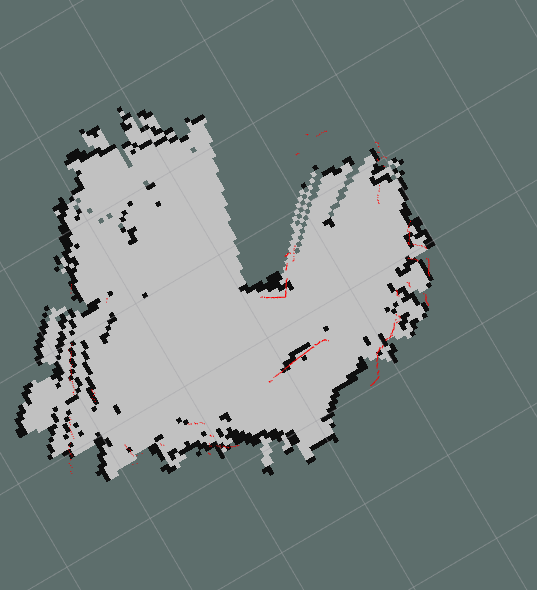
\includegraphics[width=0.6\textwidth]{img/lidarmap.png}
  \caption{Carte SLAM sans fermeture de boucle LiDAR dans RViz2}
\end{figure}

\chapter{Conclusion}

\section{Bilan}

Ce projet a permis d'améliorer la prise en main de la plateforme TurtleBot~4
ainsi que la compréhension du fonctionnement des pipelines SLAM en général. La
plateforme TurtleBot~4 s'est avérée relativement simple à prendre en main,
hormis la mise en place de l'environnement ROS. Le pipeline MC-SLAM développé
sous ROS~2 illustre la difficulté d'adaptation sur les séquences testées. Au
final, le résultat obtenu reste en deçà des attentes~: le projet s'est avéré
plus difficile que prévu et les pipelines SLAM n'ont pas pu être rendus
pleinement fonctionnels, que ce soit en RGB ou en LiDAR. En revanche, ce
travail a permis d'acquérir de nombreuses connaissances sur les algorithmes de
SLAM, la calibration multi-capteurs et les défis de l'implémentation sur une
plateforme embarquée.

\section{Perspectives}

\begin{itemize}
  \item \textbf{Finalisation du pipeline MC-SLAM}~: continuer à itérer sur les paramètres de
        l'ICP, la détection de fermeture de boucle et la fusion pour améliorer la
        précision et la robustesse.
  \item \textbf{Intégration de la caméra LWIR}~: ajouter la prise en charge de la caméra
        thermique et développer un pipeline SLAM dédié pour exploiter ses données.
  \item \textbf{Création d'un pipeline SLAM RGB complet}~: implémenter un pipeline SLAM
        visuel afin de disposer d'une comparaison réelle avec le pipeline LiDAR.
\end{itemize}

\printbibliography[heading=bibintoc, title={Références bibliographiques}]

\end{document}